\documentclass[../main.tex]{subfiles}
\graphicspath{{\subfix{../images/}}}
\begin{document}

\subsection{dataset}
This section evaluates the multipath mitigation method on the Radar Ghost Dataset \cite{ghost_dataset}. This dataset was acquired using a 77 GHz automotive radar with detection range of $0.15-153m$, azimuth field of view of $\pm70\deg$ and unambigous doppler range of $\pm44.3m/s$. The dataset includes recordings of different scenarios of outgoing/incoming VRUs progressing beside different reflectors (metal lane separators, buildings, fences, etc).

\par
The dataset is labeled and assigns a cluster ID, class and additional information about multipath targets. Only the cluster ID was used to generate real-ghost candidate pairs. Multipath information was used for validation purposes only and was not part of the method or the final evaluation process. The below table presents the results on 2 scenarios per class:

 

\begin{table}[htbp]
    \caption{Aggregation Ablation}
    \begin{center}
    \begin{tabular}{lllll}
    \hline
    \textbf{Class}                      & \textbf{MSD}                & \textbf{ANG}               &  &  \\ \hline
    \textbf{Pedestrian \#1}             & 0.0132                      & 28.09                      &  &  \\ \hline
    \textbf{Pedestrian \#2}             & 0.0223                      & 22.08                      &  &  \\ \hline
    \textbf{Cyclist \#1}                & 0.0311                      & 40.51                      &  &  \\ \hline
    \textbf{Cyclist \#2}                & 0.0327                      & 43.71                      &  &  \\ \hline
    \end{tabular}
    \end{center}
\end{table}

Overall it seems that the method performs well on both pedestrians and cyclists, and that performance is slightly better for pedestrians. A possible explanation for this performance gap stems from the difference in spatial distribution of pedestrians and cyclists. Cyclists have high variance in at least one spatial dimension while pedestrians tend to have low variance overall. fitting a linear curve to a set of low-varaince points is an easier task than trying to do the same for high-variance points, hence the better performance for pedestrians.

\par
The following sections provide detailed analysis of the results above.


\subsection{Evaluation Results - Cyclist}
Fig.~\ref{fig:cyclist} illustrates the qulitative results of using the mutlipath mitigation algorithm on a scenario where a cyclist is crossing in front of the vehicle along a small reflective wall. Fig.\ref*{fig:cyclist_metrics} depicts the quantitative metrics of the same scenario over time. \\

\par
The spread of cluster points increase with the range of the cyclist, leading to a better angular estimation when fitting the reflection line. That being said, the estimated line does not fully align with the static cluster of the actual refleciton surface. This is likely caused by imperfect assosiation between cluster points which happens due to the difference in cluster sizes (e.g. fig.~\ref{fig:cyclist}(a) where the real target cluster has 135 point while the ghost target has only 9 points).

\begin{figure}[htbp]
    \centerline{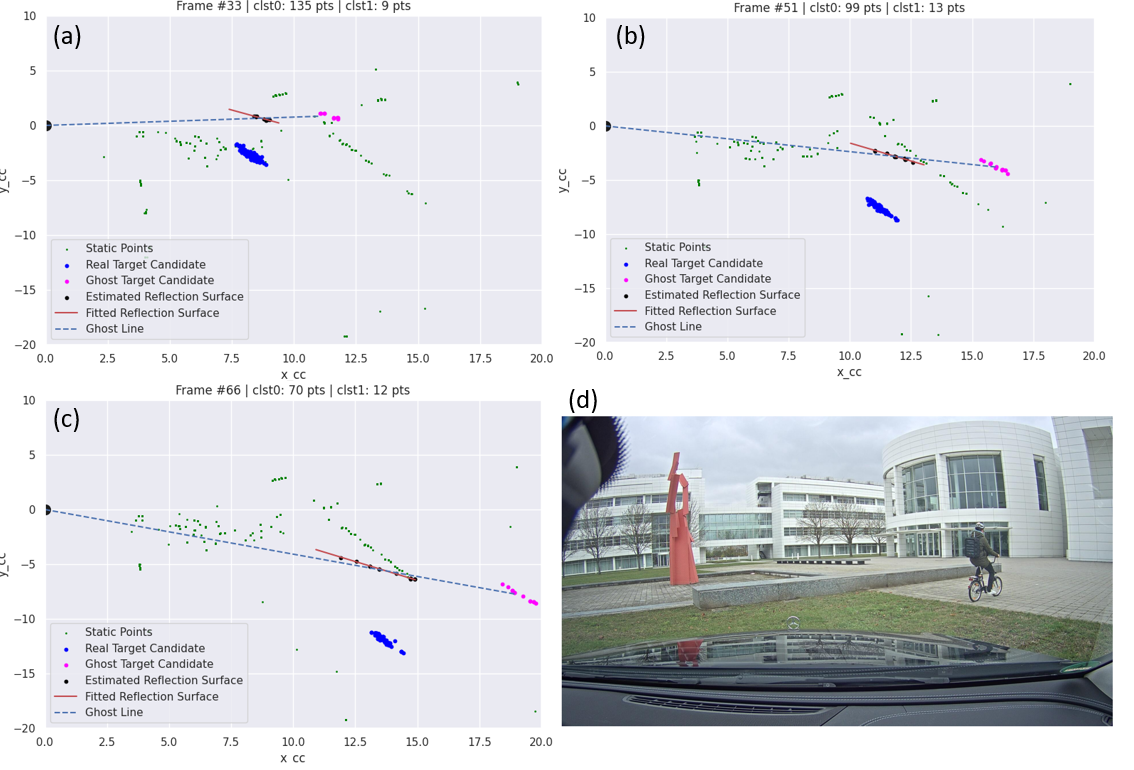
\includegraphics[scale=0.3]{figures/fig_cyclist.png}}
    \caption{(a) (b) and (c) visualize the results of the multipath mitigation method in a scenario where a cyclist is passing a small reflective wall. (d) is a camera image from that scenario.}
    \label{fig:cyclist}
\end{figure}

\begin{figure}[htbp]
    \centerline{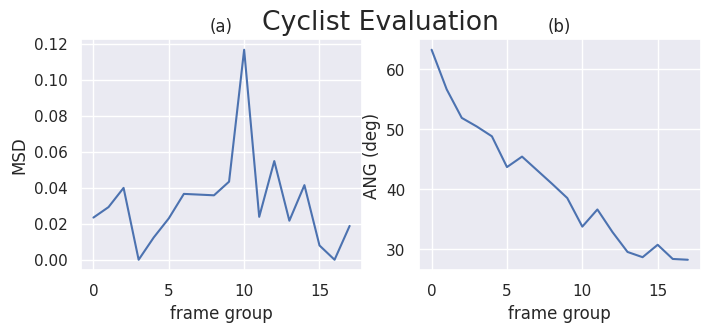
\includegraphics[scale=0.33]{figures/fig_cyclist_metrics.png}}
    \caption{Evaluation metrics for the cyclist. The x axis is the index of aggregated radar frames, and y axis is: (a) MSD. This metrics is noisey in real world scenarios. (b) ANG. This metrics improves as the cyclist drives further away from the ego vehicle.}
    \label{fig:cyclist_metrics}
\end{figure}



\subsection{Evaluation Results - Pedestrian}
Fig.~\ref{fig:ped} illustrates the qulitative results of using the mutlipath mitigation algorithm on a scenario where a pedestrian is crossing in front of the vehicle along a lane separator. Fig.\ref*{fig:ped_metrics} depicts the quantitative metrics of the same scenario over time. \\

\par
The spread of cluster points remains relatively constant for pedestrians, making the task of fitting a line to the points easier. While the metrics are quantitatively better than those of the cyclist scenarios, it is clear to see that the angle estimation for the reflection line is less than ideal. This raises the need to perhaps include neighboring static detections in the fitting process, to encourage better alignment with actual radar detections.


\begin{figure}[htbp]
    \centerline{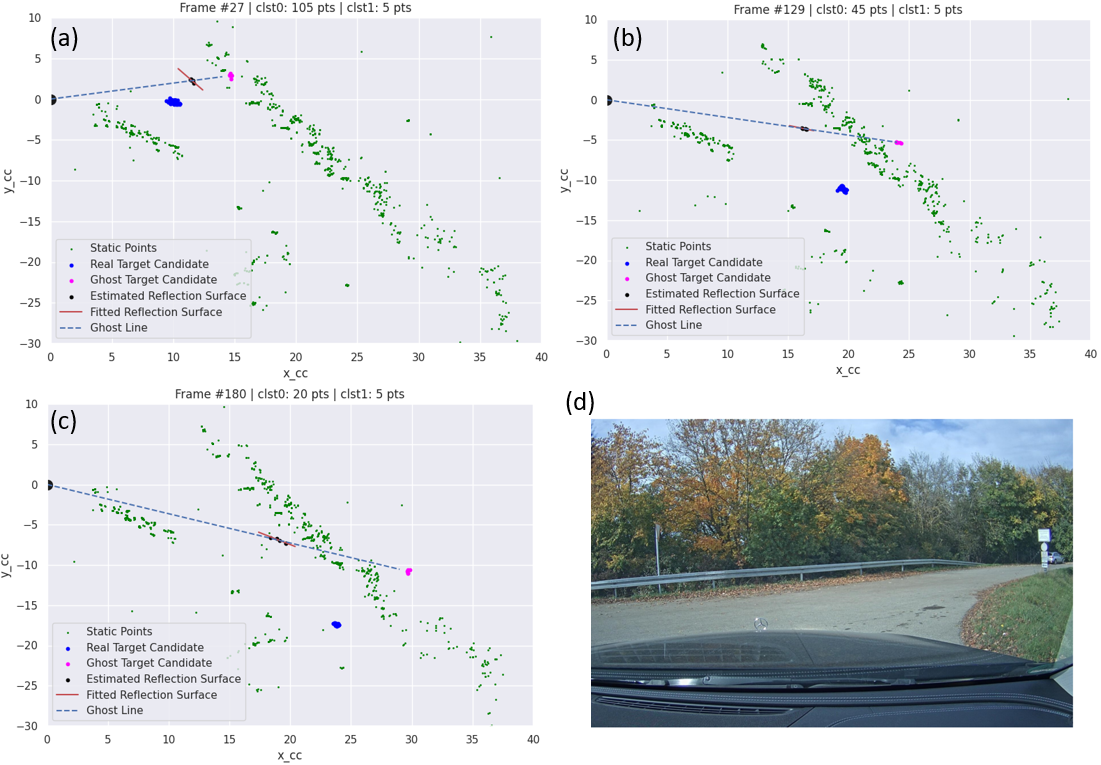
\includegraphics[scale=0.33]{figures/fig_ped.png}}
    \caption{(a) (b) and (c) visualize the results of the multipath mitigation method in a scenario where a pedestrian is walking along a lane separator. (d) is a camera image from that scenario.}
    \label{fig:ped}
\end{figure}

\begin{figure}[htbp]
    \centerline{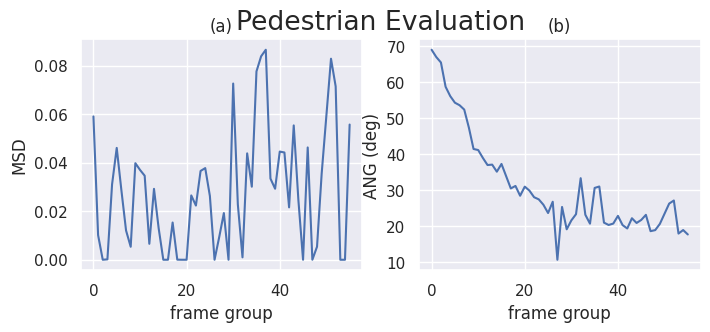
\includegraphics[scale=0.33]{figures/fig_ped_metrics.png}}
    \caption{Evaluation metrics for the cyclist. The x axis is the index of aggregated radar frames, and y axis is: (a) MSD. This metrics is noisey in real world scenarios. (b) ANG. This metrics improves as the cyclist drives further away from the ego vehicle.}
    \label{fig:ped_metrics}
\end{figure}

\subsection*{Ablation Study - Aggregation}
In order to justify the aggregation of radar point, an ablation study was conducted. The algorithm was evaluated on a pedestrian scenario with varying amounts of aggregation (0-2 frames).

\begin{table}[htbp]
    \caption{Aggregation Ablation}
    \begin{center}
    \begin{tabular}{lllll}
    \hline
    \textbf{\# of frames} & \textbf{MSD}                         & \textbf{ANG}                        &  &  \\ \hline
    \multicolumn{1}{l}{0} & \multicolumn{1}{l}{0.0275} & \multicolumn{1}{l}{32.01} &  &  \\ \cline{1-3}
    \multicolumn{1}{l}{1} & \multicolumn{1}{l}{0.0181} & \multicolumn{1}{l}{28.97} &  &  \\ \cline{1-3}
    2                       & 0.0132                      & 28.09                      &  &  \\ \hline
    \end{tabular}
    \end{center}
\end{table}

Fig.\ref*{fig:ablation} showcases the effect of frames aggreation on the ANG metrics. It is clear to see that without aggreation, estimating the correct incident angle is significantly more error-prone. Aggregating frames maintains the overall expected trend, but also alleviates the errors caused by the small number of estimated refleciton points.

\par
Depending on the required latency, one may increase aggregation in order to obtain more reliable results.

\begin{figure}[htbp]
    \centerline{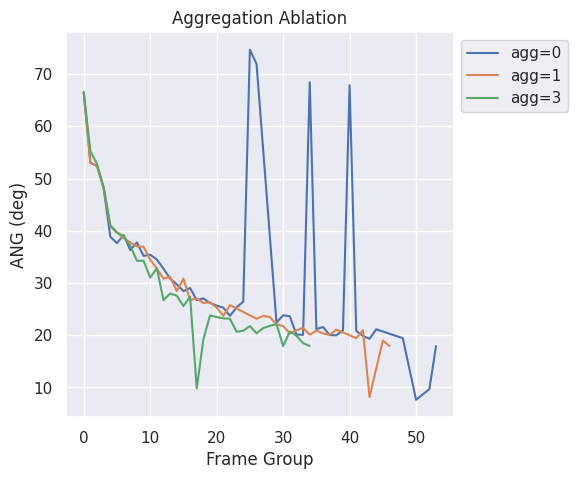
\includegraphics[scale=0.33]{figures/fig_ablation.png}}
    \caption{ANG over time for 3 levels of aggregation}
    \label{fig:ablation}
\end{figure}

\end{document}